\documentclass{standalone}

\usepackage{tikz}
\usepackage{pgfplots}

\begin{document}
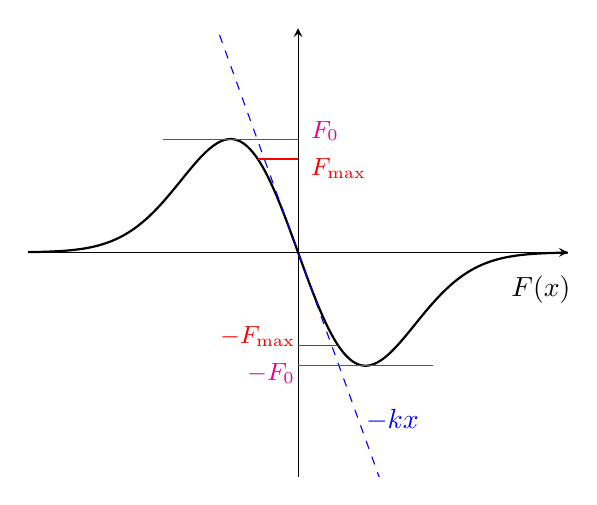
\begin{tikzpicture}
    \begin{axis}[axis lines=center, ticks=none, ymin=-1.2, ymax=1.2]
        \addplot[domain=-2:2, samples=500, thick, black]{-2*x*exp(-2*x^2)};
        \addplot[domain=-1:1, samples=500, blue, dashed]{-2*x};
        \addplot[domain=-0.3:-0, thin, red]{2*0.25};
        \node at (axis cs:1.8,-0.2){$F(x)$};
        \addplot[domain=0:0.3, thin, red]{-2*0.25};
        \node[color=blue] at (axis cs:0.7,-0.9){$-kx$};
        \node[color=red] at (axis cs:0.3,0.45){\small $F_{\max}$};
        \node[color=red] at (axis cs:-0.3,-0.45){\small $-F_{\max}$};
        \addplot[thin, magenta, domain=-1:0]{0.60653};
        \addplot[thin, magenta, domain=0:1]{-0.60653};
        \node[color=magenta] at (axis cs:0.2,0.65){\small $F_0$};
        \node[color=magenta] at (axis cs:-0.2,-0.65){\small $-F_0$};
    \end{axis}
    
\end{tikzpicture}
\end{document}